\section{ภาพรวมของระบบ}

แอปพลิเคชันสอนออกกำลังกายที่สามารถช่วยจัดท่าทางได้อย่างถูกวิธี ผู้ใช้จะเริ่มใช้งานโดยการเข้าแอปพลิเคชันบนโทรศัพท์มือถือ และเข้าสู่ระบบด้วย Username และ Password ของตนเอง เมื่อเข้าสู่ระบบเรียบร้อยแล้วจะมีหน้าแรกให้สามารถเลือกคอร์สการออกกำลังกายได้ เมื่อผู้ใช้ทำการออกกำลังกาย ในตัวแอปพลิเคชันจะเรียกใช้งาน ML Kit ซึ่งเป็น API  เกี่ยวกับการตรวจจับท่าทาง และจะเรียกข้อมูลต่าง ๆ ที่จำเป็นในการวิเคราะห์ท่าทางจาก API ในฝั่ง Back End นอกจากนี้ฟังก์ชันอื่น ๆ ของแอปพลิเคชัน เช่น ฟังก์ชันการดูกิจกรรมและตารางคะแนนลีดเดอร์บอร์ด เป็นต้น จะมีการเรียกใช้ API นี้ด้วยเช่นกัน
\\\indent
API ในฝั่ง Back End จะอยู่ในบริการของ Google Cloud Functions ซึ่งจะมีการเรียกอ่านและเก็บข้อมูลลงใน Database โดยใช้ MongoDB และเก็บข้อมูลรูปภาพหรือไฟล์ต่าง ๆ ผ่าน Google Cloud Storage
\begin{figure}
    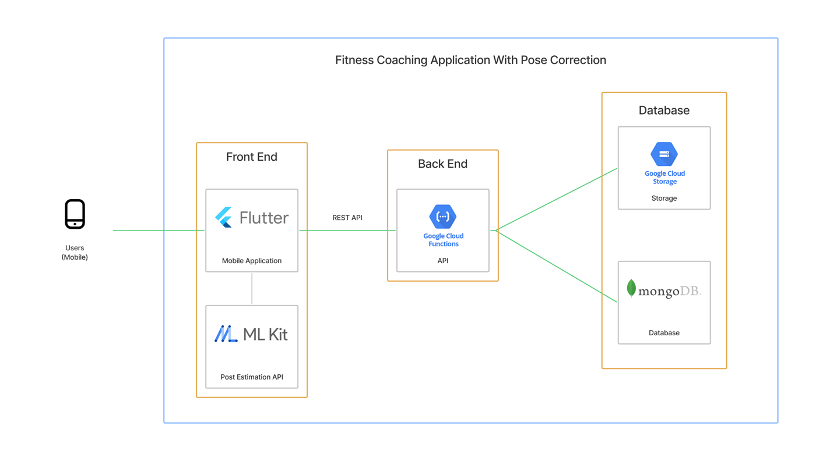
\includegraphics[width=\textwidth]{chapter_3/system overview}
    \caption{ภาพรวมระบบ}
\end{figure}